\documentclass{nime-alternate}

\begin{document}
%
% --- Author Metadata here ---
\conferenceinfo{NIME'18,}{June 3-6, 2018, Blacksburg, Virginia, USA.}

\title{Performance Systems for Live Coders and Non-Coders}

%
% You need the command \numberofauthors to handle the 'placement
% and alignment' of the authors beneath the title.
%
% For aesthetic reasons, we recommend 'three authors at a time'
% i.e. three 'name/affiliation blocks' be placed beneath the title.
%
% NOTE: You are NOT restricted in how many 'rows' of
% "name/affiliations" may appear. We just ask that you restrict
% the number of 'columns' to three.
%
% Because of the available 'opening page real-estate'
% we ask you to refrain from putting more than six authors
% (two rows with three columns) beneath the article title.
% More than six makes the first-page appear very cluttered indeed.
%
% Use the \alignauthor commands to handle the names
% and affiliations for an 'aesthetic maximum' of six authors.
% Add names, affiliations, addresses for
% the seventh etc. author(s) as the argument for the
% \additionalauthors command.
% These 'additional authors' will be output/set for you
% without further effort on your part as the last section in
% the body of your article BEFORE References or any Appendices.

\numberofauthors{4} %  in this sample file, there are a *total*
% of EIGHT authors. SIX appear on the 'first-page' (for formatting
% reasons) and the remaining two appear in the \additionalauthors section.
%
\author{
% You can go ahead and credit any number of authors here,
% e.g. one 'row of three' or two rows (consisting of one row of three
% and a second row of one, two or three).
%
% The command \alignauthor (no curly braces needed) should
% precede each author name, affiliation/snail-mail address and
% e-mail address. Additionally, tag each line of
% affiliation/address with \affaddr, and tag the
% e-mail address with \email.
%
% 1st. author
\alignauthor
Avneesh Sarwate\\
      \affaddr{Georgia Tech Center for Music Technology}\\
      \affaddr{840 McMillan Street NW}\\
      \affaddr{Atlanta, GA}\\
      \email{avneeshsarwate@gmail.com}
% 2nd. author
\alignauthor
Ryan Rose\\
      \affaddr{Georgia Tech Center for Music Technology}\\
      \affaddr{840 McMillan Street NW}\\
      \affaddr{Atlanta, GA}\\
      \email{rytrose@gatech.edu}
% 3rd. author
\alignauthor
Jason Freeman\\
      \affaddr{Georgia Tech Center for Music Technology}\\
      \affaddr{840 McMillan Street NW}\\
      \affaddr{Atlanta, GA}\\
      \email{jason.freeman@gatech.edu}
\and  % use '\and' if you need 'another row' of author names
}
% There's nothing stopping you putting the seventh, eighth, etc.
% author on the opening page (as the 'third row') but we ask,
% for aesthetic reasons that you place these 'additional authors'
% in the \additional authors block, viz.
% \additionalauthors{Additional authors: John Smith (The Th{\o}rv{\"a}ld Group,
% email: {\texttt{jsmith@affiliation.org}}) and Julius P.~Kumquat
% (K. Consortium, email: {\texttt{jpkumquat@consortium.net}}).}
% \date{30 July 1999}
% \date{30 July 1999}
% Just remember to make sure that the TOTAL number of authors
% is the number that will appear on the first page PLUS the
% number that will appear in the \additionalauthors section.

% For your initial submission you MUST ANONYMIZE the authors.

\maketitle
\begin{abstract}
This paper explores the question of how live coding musicians can perform with musicians who are not using code (such as acoustic instrumentalists or those using graphical and tangible electronic interfaces). This paper investigates performance systems that facilitate improvisation where the musicians can interact not just by listening to each other and changing their own output, but also by manipulating the data stream of the other performer(s). In a course of performance-led research four prototypes were built and analyzed using concepts from NIME and creative collaboration literature. Based on this analysis it was found that the systems should 1) provide a commonly modifiable visual representation of musical data for both coder and non-coder, and 2) provide some independent means of sound production for each user, giving the non-coder the ability to slow down and make non-realtime decisions for greater performance flexibility. 
\end{abstract}

\keywords{Live coding, creative collaboration, NIME design}

% ------- CCS Concepts
% Here is where you enter the CCS Concepts for your paper.
%
% It is strongly recommended that authors view the submission form prior to starting to write the paper, which includes information on the CCS Concepts. 
% 
%The 2012 ACM Computing Classification System (CCS) replaces the traditional 1998 version, which has served as the de facto standard classification system for the computing field. It is being integrated into the search capabilities and visual topic displays of the ACM Digital Library. Please enter the CCS XML code for the classification terms that describe your paper. To get the XML code, please use the following procedure, which is demonstrated using three NIME-related example terms: Applied computing~Sound and music computing, Applied computing~Performing arts, and Information systems~Music retrieval.
%
% 1) Browse to the website http://dl.acm.org/ccs_flat.cfm.
% 2) Select one to three classification terms from the website that describe your paper (e.g. for the example paper Applied computing~Sound and music computing, Applied computing~Performing arts, and Information systems~Music retrieval.).
% 3) For each classification you need to select the relevance (e.g. for this example, Sound and music computing is "high", Performing arts is "low", and Music retrieval is "Medium")
% 4) Once you have selected the last term, click on "view CCS Tex Code". This will generate some code, which includes some CCSXML and some lines beginning with \ccsdesc.
% 5) Keep all of this code, as you will need it for entering into the Precision Conference System paper submission form.
% 6) For this document, keep only the \ccsdesc lines. Here is what you would paste for the classification example:

\ccsdesc[500]{Applied computing~Performing arts}
\ccsdesc[500]{Applied computing~Sound and music computing}

% this line creates the CCS Concepts section.
\printccsdesc

\section{Introduction}
Live coding is an art form where performers create art through writing code in real time, often in front of an audience \cite{collins_live_2003}. Our research focuses on the interplay of two collaborating parties: live coding musicians and non-coding musicians. By non-coding musicians, we mean any musician who does not write code during a performance. In our work, non-coders have used both traditional instrument forms (e.g. guitar, keyboard) and graphical and tangible interfaces (e.g. touch screen, MIDI controller, NIMEs). We seek to design interfaces where both live coders and non-coders can contribute and interoperate in a musical performance with satisfactory knowledge of their collaborator's actions. 

To investigate interface designs that lead to successful collaboration, we conducted a program of performance-led research based on Benford et. al.'s existing methodology \cite{benford_performance-led_2013}. We developed and tested four performance interfaces (each consisting of a graphical/tangible interface for the non-coder and a live coding API in Python for the live coder), with each iteration being built off knowledge gained from performing with and analyzing the previous. Testing occurred in two forms: the authors improvised with the interfaces in an unrestricted, private setting, and also in a single public performance of semi-improvised music.

Benford et al. \cite{benford_performance-led_2013} corroborate the effectiveness of this research strategy, especially for interface design in artistic pursuits. Specifically, we employ this strategy with Benford's fifth relationship in mind: ``Theory can also guide practice, distilling artists' `craft knowledge' into guidelines that can be used by other artists or perhaps practitioners in other fields'' \cite{benford_performance-led_2013}. Our interface development highlights recurring issues in performance systems combining live coders and non-coders, for which we present potential solutions. At the time of writing, this research is exploratory and part of a larger investigation into systems that incorporate both coding and non-coding interfaces. Our current analysis finds that a commonly modifiable visual representation of musical data for both coder and non-coder greatly increases both musicians ability to communicate musical change and make informed musical decisions. Also, providing some independent means of sound production for each user gives the non-coder the ability to slow down and make non-realtime decisions, which prevents them from being overloaded by complex output from the live coder.

This paper is structured as follows: each of our prototypes' motivations are described, followed by a description of the system and its use. After testing the system through personal performance, we then analyze the successes and failures using tools from creative collaboration literature. Lastly, we synthesize the trends in our analysis into design recommendations. 

\section{Related Work}
There have been multiple systems created that explore communication between coding and non-coding musicians. One such system is Magnussons' piece Fermata, which combines the live coded Threnoscope and an augmented bass clarinet \cite{furniss_live_2016}. However, Fermata has the Threnoscope and bass clarinet operating as independent systems coordinated only by human intention rather than by some formal mechanism. We seek to incorporate a formal computational relationship between the information the two parties input into a system. Another collaborative system is Eldridge et al.'s feedback cello, in which a self-resonating cello can be live coded, but there is a strict limitation on the flexibility of the collaboration due to this being a highly-specialized instrument, both in terms of musical aesthetics and the requirement of a physically resonant instrument body \cite{eldridge_self-resonating_2017}. Other examples in live coding literature reference the ability to dynamically remap interface parameters \cite{brown_aa-cell_2007,wang_yeah_2005}, but are more focused on proving the potential of such dynamic mapping systems than analyzing the types of mappings possible. More broadly, Lee and Essl's live coded mobile music instrument successfully couples a live coder and an instrumentalist: the live-coder generates a touch-screen interface on which the non-coder performs \cite{lee_live_2013}. This collaborative experience is desirable because interacting with symbolic abstractions of musical data in real time provides the potential for deeper interaction. We seek to model this experience, but plan to focus on developing a more static interface for the non-coder.

As part of our research we analyzed our prototypes with respect to concepts from NIME and creative collaboration literature. The first is the concept of mutual engagement applied to creative collaborations proposed by Bryan-Kinns et al \cite{bryan-kinns_exploring_2007}. They define mutual engagement as the point where collaborators are ``engaged with both the product at hand and with others in the collaboration''. Bryan-Kinns et al.'s work also provides design goals for facilitating mutual engagement. We chose this framework because it studies features of realtime collaboration in the creative domain \cite{bryan-kinns_exploring_2007}. We also used Nash and Blackwell's concept of liveness in musical interfaces to investigate how coders and non-coders operate at different time scales \cite{nash_liveness_2012}. Nash defines level 3 liveness as ``edit-triggered'' systems, such as live coding, ``in which edits to the representation instantly trigger feedback, allowing users to make rapid actions and (after system response) a chance to correct mistakes'' \cite{nash_liveness_2012}. Nash then defines level 4 liveness as ``stream-driven'', such as live performance, ``in which the program is continually active, and where edits directly affect program execution, providing high visibility of the effect of actions'' \cite{nash_liveness_2012}. Nash's work provides a useful lens for examining how a live-coder and non-coder may communicate across timescales.

\section{Prototypes}
\subsection{Prototype I - Response Functions}
For our first prototype we adapted an idea from Dan Tepfer's experiments with the Yamaha Disklavier. Tepfer would play a melody on his instrument, which would be then transformed by a computer program and played to him in real-time \cite{chinen_fascinating_2017}. For Tepfer, the transformation programs were defined before the performance, and we were interested in exploring how live coding could be used to define these transformations in real-time. 

Our hypothesis was that the non-coder and live coder would pass musical material back and forth, much like jazz musicians improvising by trading fours. The non-coder would seed the system with a melody, and its transformation by the response function would provide inspiration for further content, and this cyclical process would continue.

The transformation we experimented with was buffer shuffling, i.e. permutation of sliced segments of a melody (Figure 1). To give some control over this response to the non-coding musician, we developed two different triggers that the non-coder could use to call these response functions. The first trigger activated the response function when the non-coding musician held a note longer than a specified amount of time (set by live coder). The other trigger was a specified duration of silence (also set by the live coder). Only one type of trigger could be active at a time, determined by the live coder. To implement this system we used a Novation Launchpad as a ``keyboard'', which the non-coder would play on as a typical note-triggering MIDI interface. 

\begin{figure}[htbp]
	\centering
		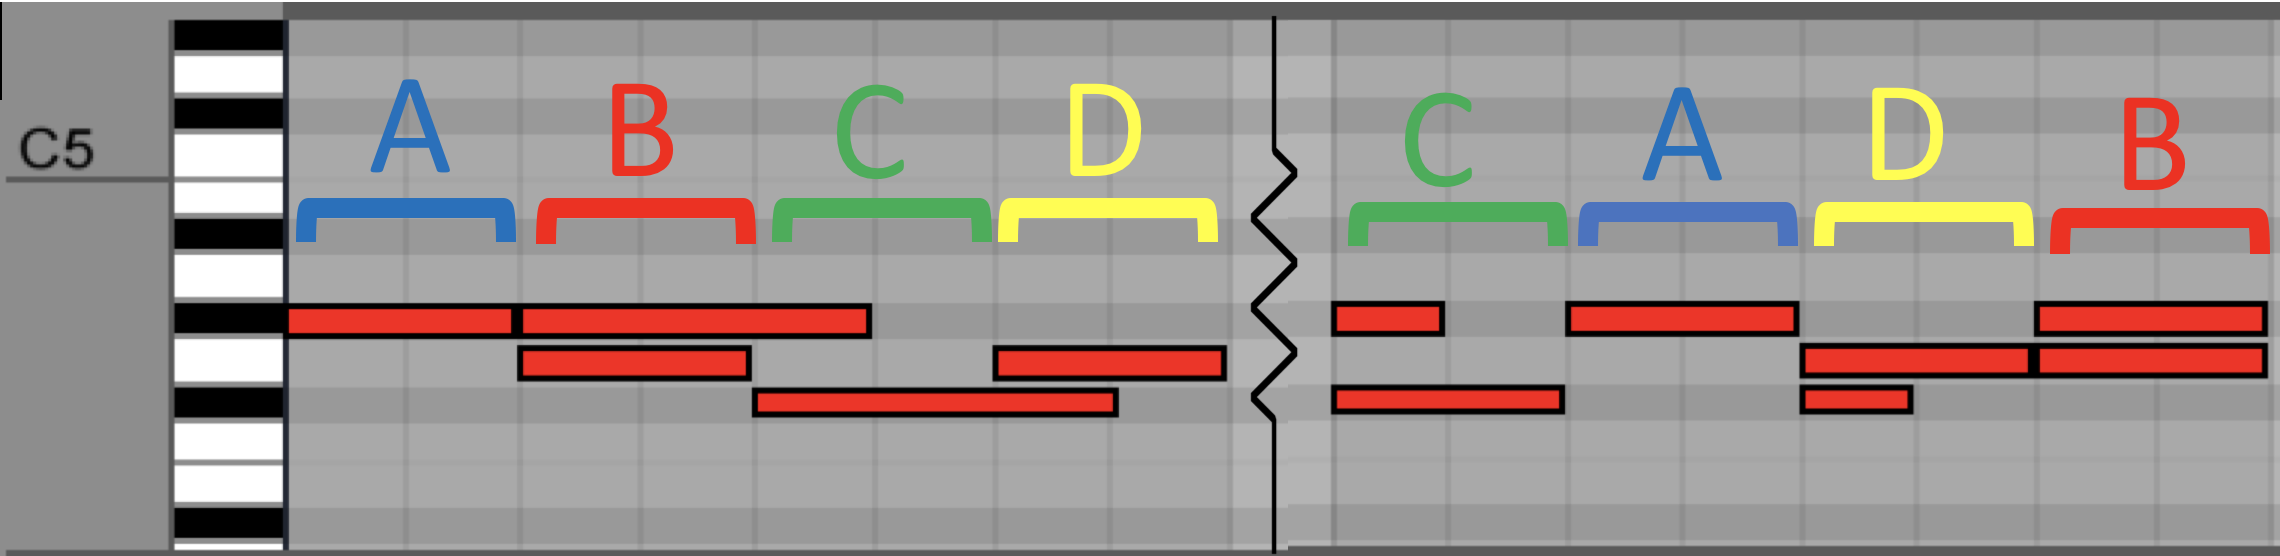
\includegraphics[width=1\columnwidth]{BufferShuffling2}
	\caption{An example of buffer shuffling. The pattern \texttt{"ABCD"} becomes \texttt{"CADB"}.}
	\label{fig:BufferShuffling2}
\end{figure}

In practice, the actions of the live coder proved too complex for the non-coder to decipher and respond to. The keyboard player (non-coder) couldn't decipher complex shufflings at all, and for simpler shufflings, they still couldn't understand them fast enough to respond quickly to changes in the pattern. In terms of Nash's levels of liveness, the live coder is engaging in a level 3 activity, and has time to produce complex output. The non-coder, as a level 4 real-time performer, is forced to parse the complex output of the live coder on the fly. Furthermore, the live coder can use the code as a visual aid when constructing the permutation. The non-coder has no visual reference at all. In terms of mutual engagement, this violates Bryan-Kinns et al.'s guideline that collaborators should share a consistent representation of the object being manipulated, in this case, music. These difficulties were exacerbated by the fact that a musical permutation is not a structure that the performers were musically familiar with, and thus had more trouble thinking about than common structures such as loops.

\subsection{Prototype II - Loop Sequencer}
Inspired by the deficiencies of the previous system, we hypothesized that a system with clearer visualized musical data, represented with more familiar metaphors, would be more successful.

For this prototype's non-coding interface we implemented a step sequencer, where each step is a measure-long melody. These melodies are recorded in real-time via MIDI controller. The system provides an optional metronome track, to facilitate real-time melody recording. The step sequencer interface was a traditional toggle grid, implemented on a Novation Launchpad. 

The live coder had the power to manipulate the sequencer grid as well as apply transformations to the recorded melodies. The transformations were the counterpoint transforms of inversion, retrograde, and transposition. With the ability to apply and undo these transformations at will, the live coder could contribute to the musical output of performances independent of the actions of the non-coder. This independence was lacking in the previous prototype.

We found performance with this system more engaging than with the previous. While performing we had better understanding of each other's actions, and could modify each other's musical output more effectively. Instead of the constant call-and-response of the previous prototype, this system provided a persistent structure (a melody loop) that did not require continuous activity to generate musical output. This allowed the non-coder to have both level 4 liveness activity (e.g. improvising on the keyboard over the sequenced melodies) and level 3 liveness activity (e.g. setting the sequencer arrangement, planning new melodies to record).

Furthermore, the visualization of a common representation led to well-informed decision-making by the performers. The step sequencer interface implemented Nielsen's heuristic of a highly visible system state, which clearly communicates what was happening musically \cite{nielsen_heuristic_1994}. Because both performers were working with the same representation and manipulating the same objects, modification of each other's output through the step sequencer was facilitated, meeting Bryan-Kinns et al.'s guideline of mutual modifiability. For the performers, looping melodies were easier to reason with than abstract musical permutations.

However, the visualization did not extend to the live coder's transformation of the non-coder's melodies. While the persistence of the loop allowed the non-coder to parse the transformation aurally over multiple loop playbacks, this added avoidable processing time. Here, mutual modifiability on the loop level was not achieved, as the transformations were not removable by the non-coder. This could have been ameliorated through a simple undo/redo button for the non-coder.

\subsection{Prototype III - Parameter Curves}
Drawing on the success of visualization from the previous interface, we were motivated to create a system with \textit{all} musical data visualized. Additionally, we wanted to explore how a live coder could interact with an audio signal from a more traditional instrument. This prototype introduces a parameter curve system, where the live coder could define curve functions of varying complexity, and map these curves to parameters on a signal processing effect chain through which the non-coder (an electric guitarist) is playing. Because curves can be easily visualized, we hypothesized that full exposure of state would lead to musically rich output. 

The signal chain consisted of a grain delay, a conventional delay, a pitch shifting module, and reverb. In an attempt to not overwhelm the guitarist with too much parameter change, only two parameters of these effects were ever being dynamically manipulated at one time. We designed a visualization where at least one period of the curve function would be shown, and a tracking line would move across time to show the current level of the effect (Figure 2).

\begin{figure}[htbp]
	\centering
		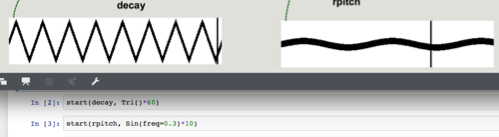
\includegraphics[width=1\columnwidth]{CurveVisualization}
	\caption{Curve visualization and code snippet from the Parameter Curves interface.}
	\label{fig:CurveVisualization}
\end{figure}

While our visual interface properly communicated relative effect values, this continuous-valued effects parameter notation was very non-standard and challenging for the guitarist to make sense of musically. Through this prototype's design process, we discovered that there is a key difference between being understandable as an interface, and being understandable in a musical sense. This is illuminated when examining this interface through the lens of liveness: much like the first interface, the live coder, operating at level 3 timescale, is creating a complex object (the curve envelope) that the guitarist must respond to at a level 4 timescale. In this instance, the object was not intuitively understood because parameter curves are not a structure that guitarists are familiar with. The usefulness of the visualization was thus lost, due to the type of information conveyed.

Furthermore, the interface violated the consistent representation feature of Bryan-Kinns' mutual engagement. The continuous parameter curve provided to the guitarist was incongruous with the discrete note data they were producing. A more successful system could have matched the data forms: displaying a stream of chords to a guitarist playing notes, or giving parameter curves to a musician controlling the knobs of a modular synthesizer. 

Lastly, this prototype suffered from the same problem for the live coder as the Response Functions system: input from the non-coder was required for the live coder to affect output. Again, the non-coder struggled to generate material, which limited live coder contribution as well.

\subsection{Prototype IV - Orbit Environment}
For our final interface, we sought to fix issues from the previous systems by designing the graphical interface and live coding API in tandem rather than adding live coding to an existing, non-coded system. In addition, we wanted to experiment with a procedural system that would lend itself to a high degree of visibility for the non-coder. To meet these constraints, we implemented a live coded physics environment where sound was generated by moving balls passing through positional triggers. A combination of touch screen and MIDI controller input allowed the non-coder to adjust the trajectory of these balls, which traveled in periodic paths across the environment. The live coder positioned lines across the environment, which triggered a note when crossed by a ball. The musical mappings of the notes triggered were defined by the live coder. The non-coder could manipulate global effects (e.g. bit-crushing, filtering, delay) through a separate, smaller, ball environment. In this environment, each ball was mapped to a different parameter, and the value of the parameter was defined by the distance of the ball from the center of the environment (Figure 3).

\begin{figure}[htbp]
	\centering
		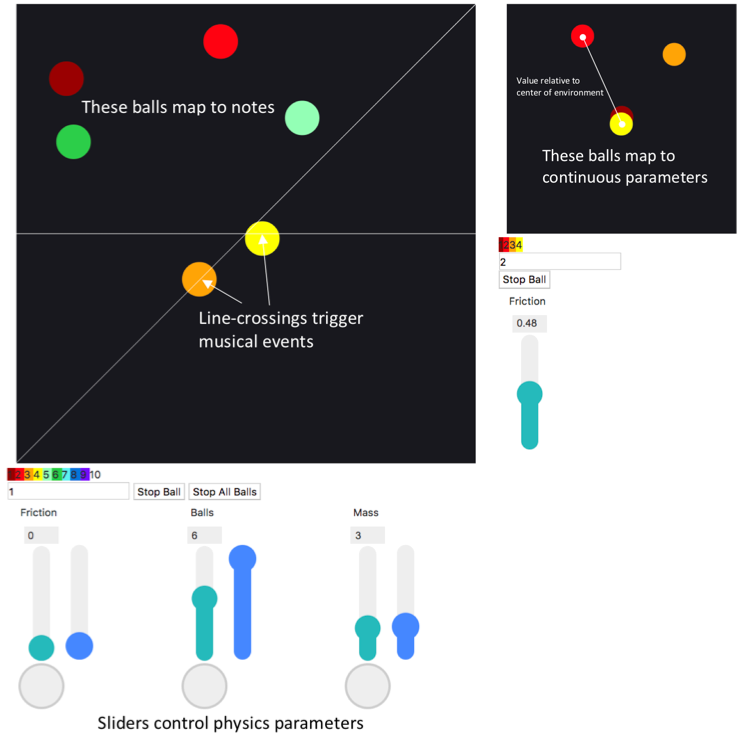
\includegraphics[width=1\columnwidth]{OrbitEnvironment2}
	\caption{The Orbit Environment interface.}
	\label{fig:OrbitEnvironment2}
\end{figure}

This system succeeded in giving the non-coder the flexibility to operate on level 3 or level 4 timescales, much like the Loop Sequencer, and allowed the coder to manipulate sound without being dependent on the level 4 actions of the non-coder. However, the system representation was musically non-standard and limited the ability of the performers to make sense of the music. For example, due to the geometry of the physics environment, it was difficult to predict the rhythmic paths of the balls, even though they were operating periodically. 

The parameters of this system were not mutually editable. Though both parties had control over system parameters, they could not effectively control each other's parameters. This prevents even the mirroring of behavior between parties, a detriment to mutual engagement as noted by Bryan-Kinns et al. Furthermore, the physics environment's rules were too complex to allow any action to have a fully predictable outcome. A performer is unable to influence another for two reasons: first, as mentioned, they don't have access to the other's parameters. Second, the system is too complex to compensate the actions of the other performer with their own. For example, if the non-coder set a ball trajectory and the live coder wanted to implement a specific change to the rhythm generated by that ball, the live coder would have to change a different parameter than the ball trajectory directly. The live coder would need to move the trigger line to compensate - an action too complex to apply accurately. This lack of mutual modifiability led to musically directionless performances.
Finally, the system lacked visualization of the musical mappings for the non-coder. While the live coder could reference the code as was possible in the Response Function system, the non-coder only had aural access to the mappings. The result was a high memory load for the non-coder \cite{nielsen_heuristic_1994}, which made the level 4 action of planning note triggers exceedingly difficult.

\section{Discussion}
\subsection{Common Design Challenges}
Two main design issues revealed themselves repeatedly through the analysis of our prototypes. The first related to the translation of musical data: if the musical representation of the live coder's actions was not immediately understandable to the non-coder, formulating a musical response was difficult as the non-coder had to first process the representation. This surfaced in the response functions of the first prototype, the parameter curves of the third, and the physics parameters of the fourth. The second prototype avoided this issue of musical representation through an intuitive visualization of musical data via the loop sequencer.

The second issue arose from complications of the performers operating on different timescales. The live coder was often able to take time to produce complex musical output, which the non-coder was forced to respond to immediately for output of the system to continue. This was prevalent again in the struggles of the non-coder using prototype I and prototype III. Both the second and the fourth prototypes avoided this by making sound generation not directly dependent on level 4 liveness input from the non-coder (e.g. in prototype II loops playback without input, and in prototype IV balls move autonomously triggering notes).

Based on these common problems and instances of their mitigation, we propose the following two design guidelines.

\subsection{Mutually Modifiable Visual Representations}
Musical state should be represented visualized in a mutually modifiable interface with musical representations intuitively familiar to the performers (particularly the non-coder). Mutual modifiablity of a common representation allows both performers to directly modify the musical output of a collaborator, rather than being forced to ``compensate'' for the change in one set of parameters by changing a different set of parameters. Furthermore, selecting a representation that is familiar to both performers allows them to respond quickly to musical changes. Familiar representation is particularly important for the non-coder, as an unfamiliar representation could hamper their ability to informedly respond to musical change in real time.

\vfill\null

\subsection{Independent Sound Generation}
The live coder and non-coder should have some independent methods for generating sound. By allowing the live coder to control the manipulation of sound without constant input from the non-coder, the non-coder is free to engage in non-real time activity, thus expanding the scope of actions that they can take during the performance. This also prevents either performer from being unable to generate music due to the inactivity of their collaborator.  


% \subsection{Tables}
% Because tables cannot be split across pages, the best
% placement for them is typically the top of the page
% nearest their initial cite.  To
% ensure this proper ``floating'' placement of tables, use the
% environment \textbf{table} to enclose the table's contents and
% the table caption.  The contents of the table itself must go
% in the \textbf{tabular} environment, to
% be aligned properly in rows and columns, with the desired
% horizontal and vertical rules.  Again, detailed instructions
% on \textbf{tabular} material
% is found in the \textit{\LaTeX\ User's Guide}.

% Immediately following this sentence is the point at which
% Table~\ref{tab:frequency} is included in the input file; compare the
% placement of the table here with the table in the printed
% dvi output of this document. 

% To get correct numbering of tables, please use the \textbf{label} command inside the \textbf{table} environment and a corresponding \textbf{ref} in the text.

% \begin{table}
% \centering
% \caption{Frequency of Special Characters}
% \begin{tabular}{|c|c|l|} \hline
% Non-English or Math&Frequency&Comments\\ \hline
% \O & 1 in 1,000& For Swedish names\\ \hline
% $\pi$ & 1 in 5& Common in math\\ \hline
% \$ & 4 in 5 & Used in business\\ \hline
% $\Psi^2_1$ & 1 in 40,000& Unexplained usage\\
% \hline\end{tabular}
% \label{tab:frequency}
% \end{table}

% To set a wider table, which takes up the whole width of
% the page's live area, use the environment
% \textbf{table*} to enclose the table's contents and
% the table caption.  As with a single-column table, this wide
% table will ``float" to a location deemed more desirable.
% Immediately following this sentence is the point at which
% Table 2 is included in the input file; again, it is
% instructive to compare the placement of the
% table here with the table in the printed dvi
% output of this document.


% \begin{table*}[htbp]
% \centering
% \caption{Some Typical Commands}
% \begin{tabular}{|c|c|l|} \hline
% Command&A Number&Comments\\ \hline
% \texttt{{\char'134}alignauthor} & 100& Author alignment\\ \hline
% \texttt{{\char'134}numberofauthors}& 200& Author enumeration\\ \hline
% \texttt{{\char'134}table}& 300 & For tables\\ \hline
% \texttt{{\char'134}table*}& 400& For wider tables\\ \hline\end{tabular}
% \end{table*}
% % end the environment with {table*}, NOTE not {table}!

% \subsection{Figures}
% Like tables, figures cannot be split across pages; the best placement for them is typically the top or the bottom of the page nearest their initial cite. To ensure this proper ``floating'' placement of figures, use the environment \textbf{figure} to enclose the figure and its caption. Optionally, for small figures that you want to place inline with the text, you can use the \textbf{htbp} options to \textbf{figure} to see whether there is space for placing it inline with the text.

% This sample document contains examples of \textbf{.pdf} (Figure~\ref{fig:BlockDiagram1}) and \textbf{.jpg} files to be displayable with \LaTeX. More details on each of these is found in the \textit{Author's Guide}.

% \begin{figure}[htbp]
% 	\centering
% 		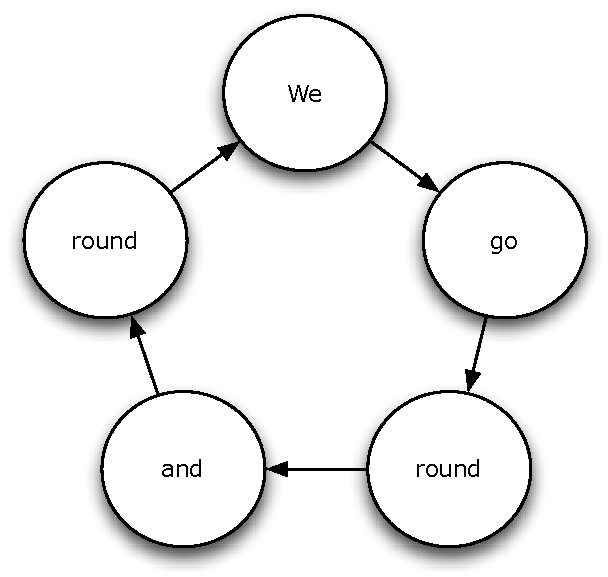
\includegraphics[width=1\columnwidth]{BlockDiagram1}
% 	\caption{A sample image in PDF format.}
% 	\label{fig:BlockDiagram1}
% \end{figure}

% As was the case with tables, you may want a figure that spans two columns (Figure~~\ref{fig:BlockDiagram2}). To do this, and still to ensure proper ``floating'' placement of tables, use the environment \textbf{figure*} to enclose the figure and its caption. And don't forget to end the environment with {figure*}, not {figure}!

% \begin{figure*}[htbp]
% 	\centering
% 		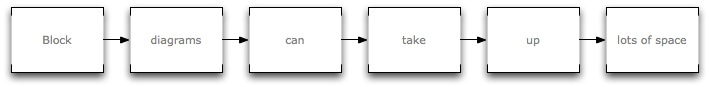
\includegraphics[width=1\textwidth]{BlockDiagram2}
% 	\caption{A sample black and white graphic (.jpg format) that needs to span two columns of text.}
% 	\label{fig:BlockDiagram2}
% \end{figure*}

% \subsection{Math Equations}
% You may want to display math equations in three distinct styles:
% inline, numbered or non-numbered display.  Each of
% the three are discussed in the next sections.

% \subsubsection{Inline (In-text) Equations}
% A formula that appears in the running text is called an
% inline or in-text formula.  It is produced by the
% \textbf{math} environment, which can be
% invoked with the usual \texttt{{\char'134}begin. . .{\char'134}end}
% construction or with the short form \texttt{\$. . .\$}. You
% can use any of the symbols and structures,
% from $\alpha$ to $\omega$, available in
% \LaTeX \cite{Lamport:LaTeX}; this section will simply show a
% few examples of in-text equations in context. Notice how
% this equation: \begin{math}\lim_{n\rightarrow \infty}x=0\end{math},
% set here in in-line math style, looks slightly different when
% set in display style.  (See next section).

% \subsubsection{Display Equations}
% A numbered display equation -- one set off by vertical space
% from the text and centered horizontally -- is produced
% by the \textbf{equation} environment. An unnumbered display
% equation is produced by the \textbf{displaymath} environment.

% Again, in either environment, you can use any of the symbols
% and structures available in \LaTeX; this section will just
% give a couple of examples of display equations in context.
% First, consider the equation, shown as an inline equation above:
% \begin{equation}\lim_{n\rightarrow \infty}x=0\end{equation}
% Notice how it is formatted somewhat differently in
% the \textbf{displaymath}
% environment.  Now, we'll enter an unnumbered equation:
% \begin{displaymath}\sum_{i=0}^{\infty} x + 1\end{displaymath}
% and follow it with another numbered equation:
% \begin{equation}\sum_{i=0}^{\infty}x_i=\int_{0}^{\pi+2} f\end{equation}
% just to demonstrate \LaTeX's able handling of numbering.



% \subsection{Theorem-like Constructs}
% Other common constructs that may occur in your article are
% the forms for logical constructs like theorems, axioms,
% corollaries and proofs.  There are
% two forms, one produced by the
% command \texttt{{\char'134}newtheorem} and the
% other by the command \texttt{{\char'134}newdef}; perhaps
% the clearest and easiest way to distinguish them is
% to compare the two in the output of this sample document:

% This uses the \textbf{theorem} environment, created by
% the\linebreak\texttt{{\char'134}newtheorem} command:
% \newtheorem{theorem}{Theorem}
% \begin{theorem}
% Let $f$ be continuous on $[a,b]$.  If $G$ is
% an antiderivative for $f$ on $[a,b]$, then
% \begin{displaymath}\int^b_af(t)dt = G(b) - G(a).\end{displaymath}
% \end{theorem}

% The other uses the \textbf{definition} environment, created
% by the \texttt{{\char'134}newdef} command:
% \newdef{definition}{Definition}
% \begin{definition}
% If $z$ is irrational, then by $e^z$ we mean the
% unique number which has
% logarithm $z$: \begin{displaymath}{\log e^z = z}\end{displaymath}
% \end{definition}

% Two lists of constructs that use one of these
% forms is given in the
% \textit{Author's  Guidelines}.
 
% There is one other similar construct environment, which is
% already set up
% for you; i.e. you must \textit{not} use
% a \texttt{{\char'134}newdef} command to
% create it: the \textbf{proof} environment.  Here
% is a example of its use:
% \begin{proof}
% Suppose on the contrary there exists a real number $L$ such that
% \begin{displaymath}
% \lim_{x\rightarrow\infty} \frac{f(x)}{g(x)} = L.
% \end{displaymath}
% Then
% \begin{displaymath}
% l=\lim_{x\rightarrow c} f(x)
% = \lim_{x\rightarrow c}
% \left[ g{x} \cdot \frac{f(x)}{g(x)} \right ]
% = \lim_{x\rightarrow c} g(x) \cdot \lim_{x\rightarrow c}
% \frac{f(x)}{g(x)} = 0,
% \end{displaymath}
% which contradicts our assumption that $l\neq 0$.
% \end{proof}

% Complete rules about using these environments and using the
% two different creation commands are in the
% \textit{Author's Guide}; please consult it for more
% detailed instructions.  If you need to use another construct,
% not listed therein, which you want to have the same
% formatting as the Theorem
% or the Definition \cite{salas:calculus} shown above,
% use the \texttt{{\char'134}newtheorem} or the
% \texttt{{\char'134}newdef} command,
% respectively, to create it.

% \subsection{A {\secit Caveat} for the \TeX\ Expert}
% Because you have just been given permission to
% use the \texttt{{\char'134}newdef} command to create a
% new form, you might think you can
% use \TeX's \texttt{{\char'134}def} to create a
% new command: \textit{Please refrain from doing this!}
% Remember that your \LaTeX\ source code is primarily intended
% to create camera-ready copy, but may be converted
% to other forms -- e.g. HTML. If you inadvertently omit
% some or all of the \texttt{{\char'134}def}s recompilation will
% be, to say the least, problematic.



% \subsection{Citations}
% Citations to articles \cite{bowman:reasoning,
% clark:pct, braams:babel, herlihy:methodology},
% conference proceedings \cite{clark:pct} or
% books \cite{salas:calculus, Lamport:LaTeX} listed
% in the Bibliography section of your
% article will occur throughout the text of your article.
% You should use BibTeX to automatically produce this bibliography;
% you simply need to insert one of several citation commands with
% a key of the item cited in the proper location in
% the \texttt{.tex} file \cite{Lamport:LaTeX}.
% The key is a short reference you invent to uniquely
% identify each work; in this sample document, the key is
% the first author's surname and a
% word from the title.  This identifying key is included
% with each item in the \texttt{.bib} file for your article.

% The details of the construction of the \texttt{.bib} file
% are beyond the scope of this sample document, but more
% information can be found in the \textit{Author's Guide},
% and exhaustive details in the \textit{\LaTeX\ User's
% Guide} \cite{Lamport:LaTeX} and in various online source.\footnote{See e.g. \url{http://www.bibtex.org/}.}

% This article shows only the plainest form
% of the citation command, using \texttt{{\char'134}cite}.
% This is what is stipulated in the SIGS style specifications.
% No other citation format is endorsed or supported.


% \subsection{Links}

% Links to URLs can be included using the \texttt{{\char'134}url} command. This will generate a clickable link like this: \url{http://www.nime2017.org}.

% %ACKNOWLEDGMENTS are optional
% \section{Acknowledgments}
% This section is optional; it is a location for you
% to acknowledge grants, funding, editing assistance and
% what have you.  In the present case, for example, the
% authors would like to thank Gerald Murray of ACM for
% his help in codifying this \textit{Author's Guide}
% and the \textbf{.cls} and \textbf{.tex} files that it describes.

\section{Additional Authors}
Additional authors: Jack Armitage (Centre for Digital Music, Queen Mary U of London),
email: {\texttt{j.d.k.armitage@qmul.ac.uk}}).
\date{27 January 2018}

%
% The following two commands are all you need in the
% initial runs of your .tex file to
% produce the bibliography for the citations in your paper.
\bibliographystyle{abbrv}
\bibliography{references}  % sigproc.bib is the name of the Bibliography in this case
% You must have a proper ".bib" file
%  and remember to run:
% latex bibtex latex latex
% to resolve all references
%
% ACM needs 'a single self-contained file'!
%
% %APPENDICES are optional
% \appendix
% %Appendix A
% \section{Headings in Appendices}
% The rules about hierarchical headings discussed above for
% the body of the article are different in the appendices.
% In the \textbf{appendix} environment, the command
% \textbf{section} is used to
% indicate the start of each Appendix, with alphabetic order
% designation (i.e. the first is A, the second B, etc.) and
% a title (if you include one).  So, if you need
% hierarchical structure
% \textit{within} an Appendix, start with \textbf{subsection} as the
% highest level. Here is an outline of the body of this
% document in Appendix-appropriate form:
% \subsection{Introduction}
% \subsection{The Body of the Paper}
% \subsubsection{Type Changes and  Special Characters}
% \subsubsection{Math Equations}
% \paragraph{Inline (In-text) Equations}
% \paragraph{Display Equations}
% \subsubsection{Citations}
% \subsubsection{Tables}
% \subsubsection{Figures}
% \subsubsection{Theorem-like Constructs}
% \subsubsection*{A Caveat for the \TeX\ Expert}
% \subsection{Conclusions}
% \subsection{Acknowledgments}
% This section is inserted by \LaTeX; you do not insert it.
% You just add the names and information in the
% \texttt{{\char'134}additionalauthors} command at the start
% of the document.
% \subsection{References}
% Generated by bibtex from your ~.bib file.  Run latex,
% then bibtex, then latex twice (to resolve references)
% to create the ~.bbl file.  Insert that ~.bbl file into
% the .tex source file and comment out
% the command \texttt{{\char'134}thebibliography}.

% % This next section command marks the start of
% % Appendix B, and does not continue the present hierarchy
% \section{More Help for the Hardy}
% The sig-alternate.cls file itself is chock-full of succinct
% and helpful comments.  If you consider yourself a moderately
% experienced to expert user of \LaTeX, you may find reading
% it useful but please remember not to change it.

%%% Place this command where you want to balance the columns on the last page. 
%\balancecolumns 

% That's all folks!
\end{document}
